\section*{Εισαγωγή}
\addcontentsline{toc}{section}{Εισαγωγή}

Η παρούσα εργασία αφορά τον προσδιορισμό της αεροελαστικής συμπεριφοράς διδιάστατης αεροτομής. Συγκεκριμένα, θα ασχοληθούμε με τον προσδιορισμό της αεροδυναμικής απόσβεσης και τη χρονική απόκριση της αεροτομής σε ελεύθερο πεδίο ροής. Η αεροδυναμική μοντελοποίηση της αεροτομής θα γίνει με δύο διαφορετικές μεθόδους, θεωρώντας μόνιμη και αποκατεστημένη ροή, και χρησιμοποιώντας μη-μόνιμο μοντέλο που λαμβάνει υπόψη και μεταβατικά φαινόμενα, ωστόσο περεταίρω εξήγηση δίνεται στις παρακάτω παραγράφους. Αναφορικά με την ελαστική στήριξη της αεροτομής, θεωρούμε τμήμα (μοναδιαίου μήκους) μιας πτέρυγας, και η ελαστική στήριξη αφορά την ανηγμένη δυσκαμψία σε κάμψη της πτέρυγας, στη θέση του τμήματος που μελετάμε. Επιπλέον, θεωρούμε μηδενική δομική απόσβεση (structural damping) και πως οι κύριοι άξονες του μητρώου ακαμψίας της διατομής είναι προσανατολισμένοι παράλληλα, και κάθετα στην χορδή της αεροτομής (σε μηδενική γωνία δεν έχουμε ελαστική σύζευξη). Ένα απλοποιημένο σχήμα του μοντέλου φαίνεται στο σχήμα \ref{fig:sxima}. 

\begin{figure}[ht!]
    \begin{center}
        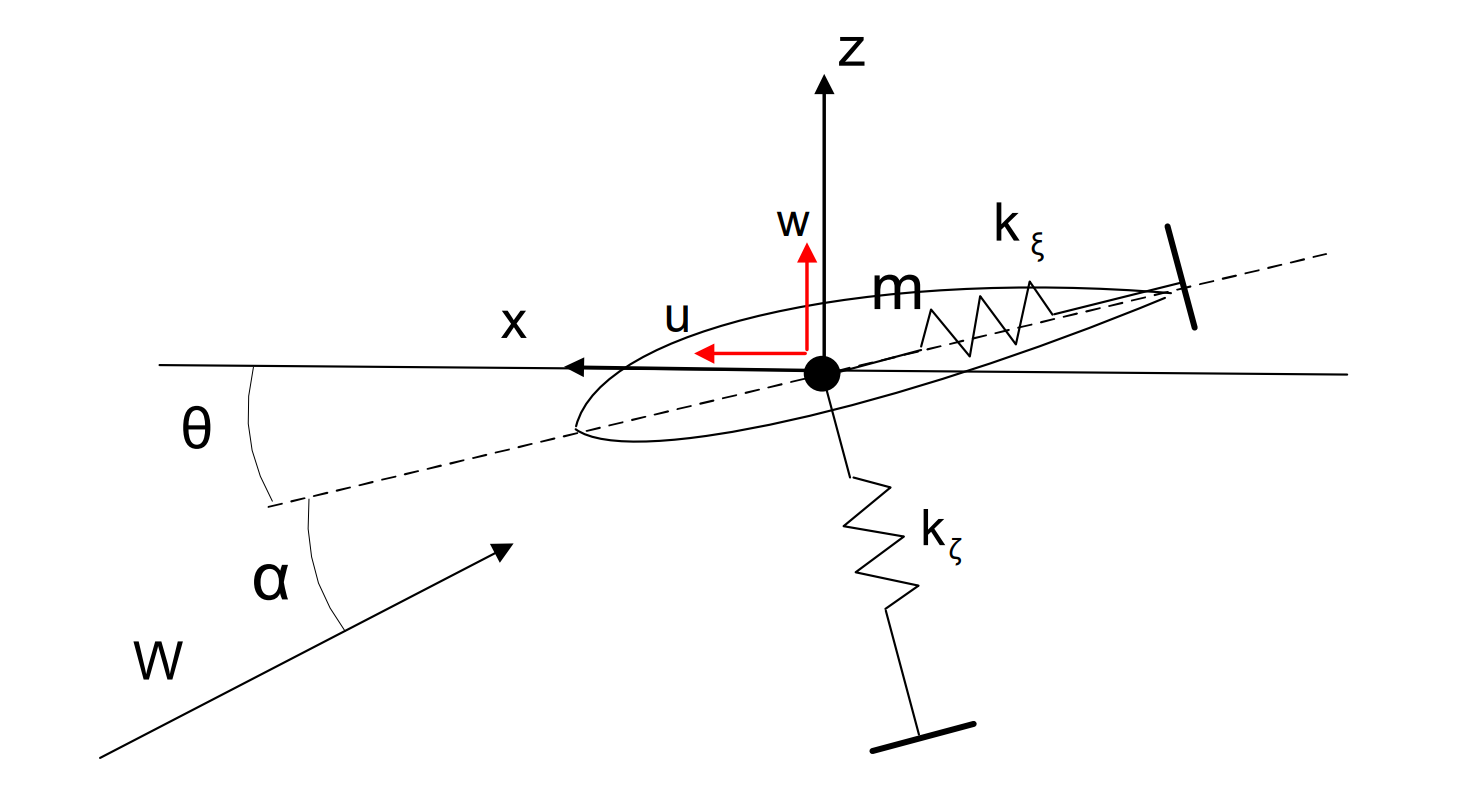
\includegraphics[width=0.85\textwidth]{./figures/sxima.png}
    \end{center}
    \caption{Σχηματική αναπαράσταση μοντέλου αεροτομής}
    \label{fig:sxima}
\end{figure}


